%! TEX program = lualatex

\documentclass[nobackground,dvipsnames,table]{beamer}
\usepackage{tsc}
\usepackage{pdfpc}
\usepackage{pgfpages}
\usepackage{multimedia}
%\usepackage{sio}
\usepackage{wrapfig}

%%%%%%%% edit hyperlink colors %%%%%%%%
\hypersetup{
  colorlinks   = true, 
  urlcolor     = tscurl, % color of external hyperlinks
  linkcolor    = white,   % color of internal links
}

\mode<presentation>
{\usetheme{default}
	\usecolortheme{tsc}
	\setbeamercovered{transparent}
	\useinnertheme[shadow=false]{rounded}
	\usebackgroundtemplate{}
	\setbeamercolor*{frametitle}{parent=palette primary}
	\setbeamerfont{block title}{size={}}
	\setbeamertemplate{navigation symbols}{}
    \setbeamertemplate{itemize items}[circle]
        \setbeamertemplate{enumerate items}[circle]

}

%{\usetheme{Hannover}
%	\usecolortheme{sio}
%	\setbeamercovered{transparent}
%	\useinnertheme[shadow=false]{rounded}
%	\usebackgroundtemplate{}
%	\setbeamercolor*{frametitle}{parent=palette primary}
%	\setbeamerfont{block title}{size={}}
%	\setbeamertemplate{navigation symbols}{}
%}

%%%%%%%%%%%%%%%%%%%%%%%%%%%%%%%%%%%%%%%%%%%%%%%%
%%%%%%%%%%%%%%%%  SLIDE 1  %%%%%%%%%%%%%%%%%%%%%
%%%%%%%%%%%%%%%%%%%%%%%%%%%%%%%%%%%%%%%%%%%%%%%%
\title[Information Environment]{Information Environment}

\author[]{}
%\institute[TSC]{\large Trust \& Safety Teaching Consortium}
\date[2023]{}
\subject{Trust and Safety}

\AddToShipoutPictureBG*{
  \AtPageLowerLeft{\hspace{-0.4cm}
    
\includegraphics[width=13.1cm]{img/consortium-image}}
}
% Change this to make a file with just slides, just notes or both
%\setbeameroption{hide notes}                 % Only slides
%\setbeameroption{show only notes}            % Only notes
\setbeameroption{show notes on second screen} % Both

\begin{document}

%\coverpage

\begin{frame}
	\titlepage
\end{frame}


%%%%%%%%%%%%%%%%%%%%%%%%%%%%%%%%%%%%%%%%%%%%%%%%
%%%%%%%%%%%%%%%%  SLIDE 2  %%%%%%%%%%%%%%%%%%%%%
%%%%%%%%%%%%%%%%%%%%%%%%%%%%%%%%%%%%%%%%%%%%%%%%
\begin{frame}{Learning Objectives}

\begin{itemize}
    \item Describe different definitions of disinformation, misinformation, and propaganda
    \item Identify strategies from social media and governmental organizations for identifying, tracking misinformation.
    \item Understand the demand-side: Cognitive aspect: Why does information/rumors/ conspiracy theories resonate with individuals
    \item Examine interventions designed to mitigate misinformation
    \item Analyse the supply-side: Influence Operations / Monetary incentives of misinformation
\end{itemize}
\end{frame}

%%%%%%%%%%%%%%%%%%%%%%%%%%%%%%%%%%%%%%%%%%%%%%%%
%%%%%%%%%%%%%%%%  SLIDE 3  %%%%%%%%%%%%%%%%%%%%%
%%%%%%%%%%%%%%%%%%%%%%%%%%%%%%%%%%%%%%%%%%%%%%%%
\begin{frame}{Disinformation}

\small{
There are multiple definitions for disinformation.  The intent is to give students several and establish a framework from which to define it and categorize content.
 
For example, disinformation can be a subset of misinformation.  Under this construct disinformation is misinformation that is deliberately propagated. (Guess and Lyons)

What distinguishes disinformation from misinformation is a matter of intent. Disinformation is meant to deceive, while misinformation may be inadvertent or
Unintentional.

Other definitions for disinformation characterize it as wholly distinct from misinformation.
}

\note[]{
Guess, A. M., \& Lyons, B. A. (2020). Misinformation, disinformation, and online propaganda. \emph{Social media and democracy: The state of the field, prospects for reform, 10.} \href{https://www.cambridge.org/core/books/social-media-and-democracy/E79E2BBF03C18C3A56A5CC393698F117}{Accessible for free here.}
}
\end{frame}

%%%%%%%%%%%%%%%%%%%%%%%%%%%%%%%%%%%%%%%%%%%%%%%%
%%%%%%%%%%%%%%%%  SLIDE 4  %%%%%%%%%%%%%%%%%%%%%
%%%%%%%%%%%%%%%%%%%%%%%%%%%%%%%%%%%%%%%%%%%%%%%%
\begin{frame}{Disinformation}

Disinformation can be distinguished from misinformation using criteria.  To determine if a piece of content is disinformation or something different:
\begin{itemize}
    \item Content is disinformation when the identity of the content originator is intentionally masked; 
    \item The released information is harmful or destructive content intended to influence an outcome; 
    \item The originator has a predetermined political, military, economic, or social objective. (Murphy)
\end{itemize}

\note[]{
-Murphy, Brian J. “The Impact of Social Media Conveyed Russian-Backed Disinformation in a Polarized America: An Examination of the Executive Branch’s Ethical Responsibility to Respond.” Ph.D., Georgetown University, 2022. \href{https://www.proquest.com/docview/2760166084/abstract/9EE61E3EE4184D8BPQ/1}{https://www.proquest.com/docview/2760166084/abstract/9EE61E3EE4184D8BPQ/1}
}
\end{frame}


%%%%%%%%%%%%%%%%%%%%%%%%%%%%%%%%%%%%%%%%%%%%%%%%
%%%%%%%%%%%%%%%%  SLIDE 5  %%%%%%%%%%%%%%%%%%%%%
%%%%%%%%%%%%%%%%%%%%%%%%%%%%%%%%%%%%%%%%%%%%%%%%
\begin{frame}{Disinformation’s Three Criteria}

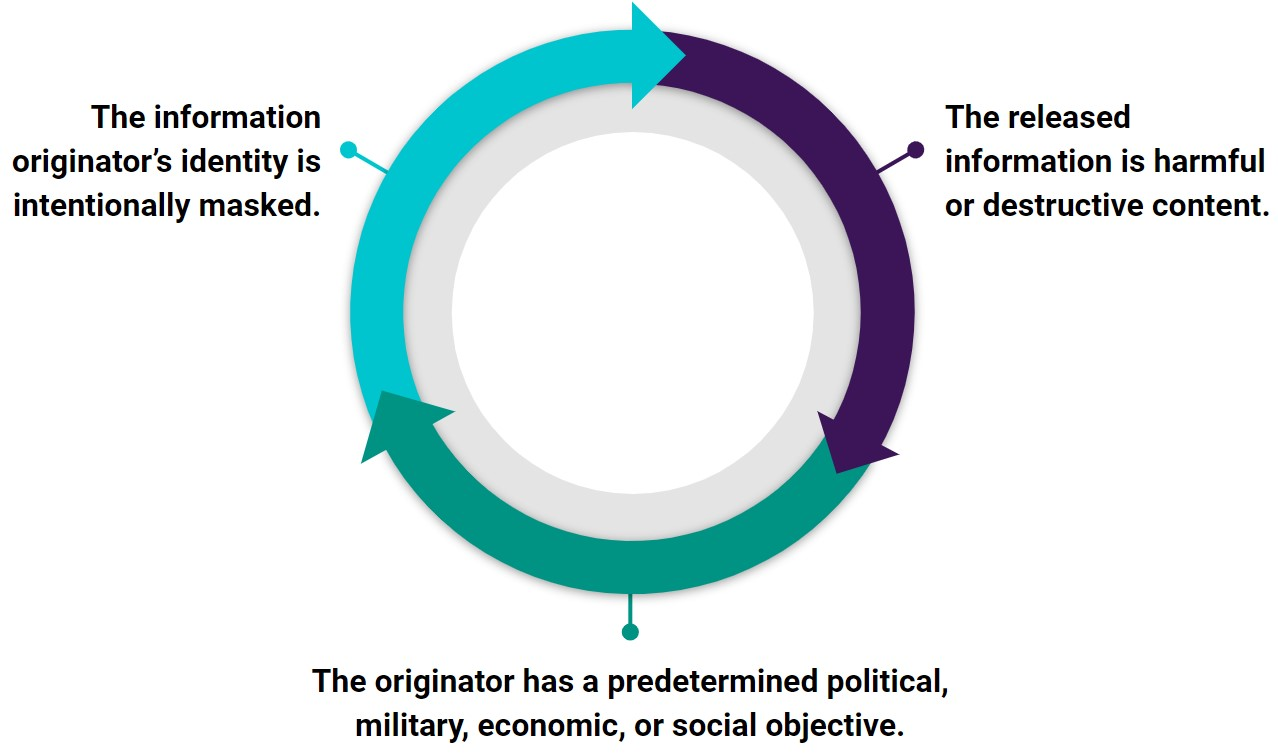
\includegraphics[width=\textwidth]{img/fig1.jpg}

\end{frame}


%%%%%%%%%%%%%%%%%%%%%%%%%%%%%%%%%%%%%%%%%%%%%%%%
%%%%%%%%%%%%%%%%  SLIDE 6  %%%%%%%%%%%%%%%%%%%%%
%%%%%%%%%%%%%%%%%%%%%%%%%%%%%%%%%%%%%%%%%%%%%%%%
\begin{frame}{Disinformation}
The fact there is no standard definition has caused confusion in research, for institutions, and among policy makers.

\begin{itemize}
    \item For instance, in August of 2022, the Department of Homeland Security’s Office of Inspector General released a reported title “DHS Needs a Unified Strategy to Disinformation Campaigns.”  The report indicated that the department lacked a coherent strategy to counter foreign and domestic-based disinformation.  Among its finding were multiple definitions for disinformation used by various DHS components. \href{https://www.oig.dhs.gov/sites/default/files/assets/2022-08/OIG-22-58-Aug22.pdf}{OIG-22-58 - DHS Needs a Unified Strategy to Counter Disinformation Campaigns}
    \item Another way to analyze the problem is to consider there is often an implied understanding when the term is used.  It is conflated in the public domain with terms such as a lie, political speech, and opinions.
\end{itemize}

\note[]{
\url{https://www.oig.dhs.gov/sites/default/files/assets/2022-08/OIG-22-58-Aug22.pdf} (OIG-22-58 - DHS Needs a Unified Strategy to Counter Disinformation Campaigns)
}
\end{frame}


%%%%%%%%%%%%%%%%%%%%%%%%%%%%%%%%%%%%%%%%%%%%%%%%
%%%%%%%%%%%%%%%%  SLIDE 7  %%%%%%%%%%%%%%%%%%%%%
%%%%%%%%%%%%%%%%%%%%%%%%%%%%%%%%%%%%%%%%%%%%%%%%
\begin{frame}{Misinformation}
The various definitions for misinformation are more similar than different:  

\begin{itemize}
    \item Misinformation is defined as conveying information constituting a claim that contradicts or distorts common understandings of verifiable facts. (Guess and Lyons)
    \item The intent behind transmitting the factually inaccurate content is inadvertent or unintentional.
    \item When discussing misinformation there are epistemological questions that can weaken any definition.  For example, evaluating its relationship to a lie or determining what makes up a fact are just some of them.
\end{itemize}

\note[]{
-Guess, A. M., \& Lyons, B. A. (2020). Misinformation, disinformation, and online propaganda. \emph{Social media and democracy: The state of the field, prospects for reform, 10.} \url{https://www.cambridge.org/core/books/social-media-and-democracy/E79E2BBF03C18C3A56A5CC393698F117} \newline \newline 
-Wardle, Claire, and Hossein Derakhshan. “Thinking about ‘Information Disorder’: Formats of Misinformation, Disinformation, and Mal-Information.” In \emph{Journalism, Fake News \& Disinformation: Handbook for Journalism Education and Training,} 43–54. Paris: UNESCO, 2018. 

}
\end{frame}


%%%%%%%%%%%%%%%%%%%%%%%%%%%%%%%%%%%%%%%%%%%%%%%%
%%%%%%%%%%%%%%%%  SLIDE 8  %%%%%%%%%%%%%%%%%%%%%
%%%%%%%%%%%%%%%%%%%%%%%%%%%%%%%%%%%%%%%%%%%%%%%%
\begin{frame}{Propaganda}

\begin{minipage}{0.5\textwidth}
    \footnotesize{
        Like disinformation, the meaning of propaganda can vary:
        \begin{itemize}
            \item Initially, propaganda had a positive connotation.  The term gained notoriety in 1627 when Pope Urban VIII founded the College of Propaganda.  The mission of the college was to educate priests.
            \item The term became more and more associated with coercive attempts of a state to distort and manipulate information for the state's benefit.  
            \item After World War I the propaganda had become negative in meaning.
        \end{itemize}
    }
\end{minipage}
\hspace{0.05\textwidth}
\begin{minipage}{0.42\textwidth}
    
\includegraphics[width=\textwidth]{img/fig2.jpg}
\end{minipage}

\note[]{
-Murphy, Brian J. “The Impact of Social Media Conveyed Russian-Backed Disinformation in a Polarized America: An Examination of the Executive Branch’s Ethical Responsibility to Respond.” Ph.D., Georgetown University, 2022. \href{https://www.proquest.com/docview/2760166084/abstract/9EE61E3EE4184D8BPQ/1}{https://www.proquest.com/docview/2760166084/abstract/9EE61E3EE4184D8BPQ/1}
}
\end{frame}


%%%%%%%%%%%%%%%%%%%%%%%%%%%%%%%%%%%%%%%%%%%%%%%%
%%%%%%%%%%%%%%%%  SLIDE 9  %%%%%%%%%%%%%%%%%%%%%
%%%%%%%%%%%%%%%%%%%%%%%%%%%%%%%%%%%%%%%%%%%%%%%%
\begin{frame}{Propaganda}

\begin{itemize}
    \item One definition for propaganda is "information that can be true but is used to 'disparage opposing viewpoints.'" (Guess and Lyons)
    \item Another is it is the "systematic dissemination of information for control, especially biased or misleading, promotes a political cause or point of view.  All propaganda contains inherent epistemic defects." (Murphy)
    \item Disinformation the sender's identity is masked.  Not necessarily the case for propaganda
    \item Disinformation is designed to be disruptive.  Propaganda is intended to exert control.
    \item Propaganda and misinformation are different based on the intent of the sender.
\end{itemize}

\note[]{
Guess, A. M., \& Lyons, B. A. (2020). Misinformation, disinformation, and online propaganda. \emph{Social media and democracy: The state of the field, prospects for reform, 10.} \href{https://www.cambridge.org/core/books/social-media-and-democracy/E79E2BBF03C18C3A56A5CC393698F117}{Accessible for free here.} \newline
\newline 
-Murphy, Brian J. “The Impact of Social Media Conveyed Russian-Backed Disinformation in a Polarized America: An Examination of the Executive Branch’s Ethical Responsibility to Respond.” Ph.D., Georgetown University, 2022. \href{https://www.proquest.com/docview/2760166084/abstract/9EE61E3EE4184D8BPQ/1}{https://www.proquest.com/docview/2760166084/abstract/9EE61E3EE4184D8BPQ/1}
}
\end{frame}


%%%%%%%%%%%%%%%%%%%%%%%%%%%%%%%%%%%%%%%%%%%%%%%%
%%%%%%%%%%%%%%%%  SLIDE 10  %%%%%%%%%%%%%%%%%%%%%
%%%%%%%%%%%%%%%%%%%%%%%%%%%%%%%%%%%%%%%%%%%%%%%%
\begin{frame}{Class Questions}

\begin{minipage}{0.46\textwidth}
    \small{
        Disinformation vs. Misinformation vs. Propaganda.
        \begin{itemize}
            \item Have all three been around since humans could speak?
            \item Has the social media age made the terms more potent?
            \item Why have the terms become political?
        \end{itemize}
    }
\end{minipage}
\hspace{0.05\textwidth}
\begin{minipage}{0.47\textwidth}
\tiny{
    Additional Reading:
    Murphy, Brian J. “The Impact of Social Media Conveyed Russian-Backed Disinformation in a Polarized America: An Examination of the Executive Branch’s Ethical Responsibility to Respond.” Ph.D., Georgetown University, 2022. \href{https://www.proquest.com/docview/2760166084/abstract/9EE61E3EE4184D8BPQ/1}{Accessible here.}, 8-25 \newline 
    
    Lazer, D. M., Baum, M. A., Benkler, Y., Berinsky, A. J., Greenhill, K. M., Menczer, F., ... \& Zittrain, J. L. (2018). The science of fake news. \emph{Science}, 359(6380), 1094-1096. \href{https://www.science.org/doi/full/10.1126/science.aao2998}{Accessible for free here.} \newline 
    
    Wardle, Claire, and Hossein Derakhshan. “Thinking about ‘Information Disorder’: Formats of Misinformation, Disinformation, and Mal-Information.” In \emph{Journalism, Fake News \& Disinformation: Handbook for Journalism Education and Training}, 43–54. Paris: UNESCO, 2018. 
}
\end{minipage}
\end{frame}

%%%%%%%%%%%%%%%%%%%%%%%%%%%%%%%%%%%%%%%%%%%%%%%%
%%%%%%%%%%%%%%%%  SLIDE 11  %%%%%%%%%%%%%%%%%%%%%
%%%%%%%%%%%%%%%%%%%%%%%%%%%%%%%%%%%%%%%%%%%%%%%%
\begin{frame}{}

\begin{minipage}{0.4\textwidth}
    \raggedright\Large{\textbf{Strategies from social media and governmental organizations for identifying, tracking and countering mis and disinformation.}}
\end{minipage}
\hspace{0.05\textwidth}
\begin{minipage}{0.5\textwidth}

    \begin{itemize}
    \small{
        \item Countries on the periphery of authoritarian nations have come up with strategies to spot mis and disinformation.
        \item Just a few of them are: Estonia, Lithuania, Finland, and Sweden
        \item One thing they share in common is building a more resilient population
    }
    \end{itemize}
\end{minipage}
\end{frame}


%%%%%%%%%%%%%%%%%%%%%%%%%%%%%%%%%%%%%%%%%%%%%%%%
%%%%%%%%%%%%%%%%  SLIDE 12  %%%%%%%%%%%%%%%%%%%%
%%%%%%%%%%%%%%%%%%%%%%%%%%%%%%%%%%%%%%%%%%%%%%%%
\begin{frame}{Sweden}
\begin{minipage}{\textwidth}
    \centering 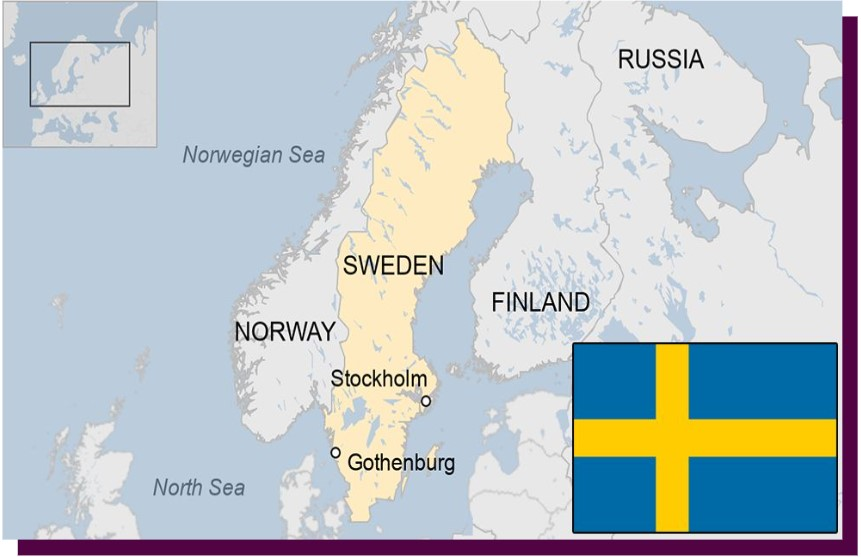
\includegraphics[scale=.35]{img/fig3.jpg}
\end{minipage}

\begin{minipage}{\textwidth}
    \footnotesize{
    \begin{itemize}
        \item Formed and budgeted for an agency called Psychological Defense Authority (PDA).
        \item The PDA serves as the single point of coordination for civil and military institutions combating Russian disinformation operations.
        \item The PDA is sensitive to losing its moral authority if it is viewed as partial or political.
        \item Independent assessments have indicated the Swedish approach is successful.  Sweden has a more media and social media literate and, therefore, resilient populace.
    \end{itemize}
    }
\end{minipage}
%\hspace{0.05\textwidth}


\note[]{
 -Niklas H. Rossbach, “Psychological Defense:  Vital for Sweden’s Capability,” \emph{Strategic Outlook 7} (November 2017), \href{https://www.foi.se/rest-api/report/FOI\%20MEMO\%206207}{https://www.foi.se/rest-api/report/FOI\%20MEMO\%206207} \newline \newline 
-Gordon LaForge, “Sweden Defends Its Elections Against Disinformation, 2016 – 2018,” Princeton University Innovations for Successful Societies, December 16, 2020, 
\href{https://successfulsocieties.princeton.edu/publications/sweden-defends-its-elections-against-disinformation-2016-\%E2\%80\%93-2018}{https://successfulsocieties.princeton.edu/publications/sweden-defends-its-elections-against-disinformation-2016-\%E2\%80\%93-2018}}
\end{frame}


%%%%%%%%%%%%%%%%%%%%%%%%%%%%%%%%%%%%%%%%%%%%%%%%
%%%%%%%%%%%%%%%%  SLIDE 13  %%%%%%%%%%%%%%%%%%%%%
%%%%%%%%%%%%%%%%%%%%%%%%%%%%%%%%%%%%%%%%%%%%%%%%
\begin{frame}{Finland}
\begin{minipage}{\textwidth}
    \centering 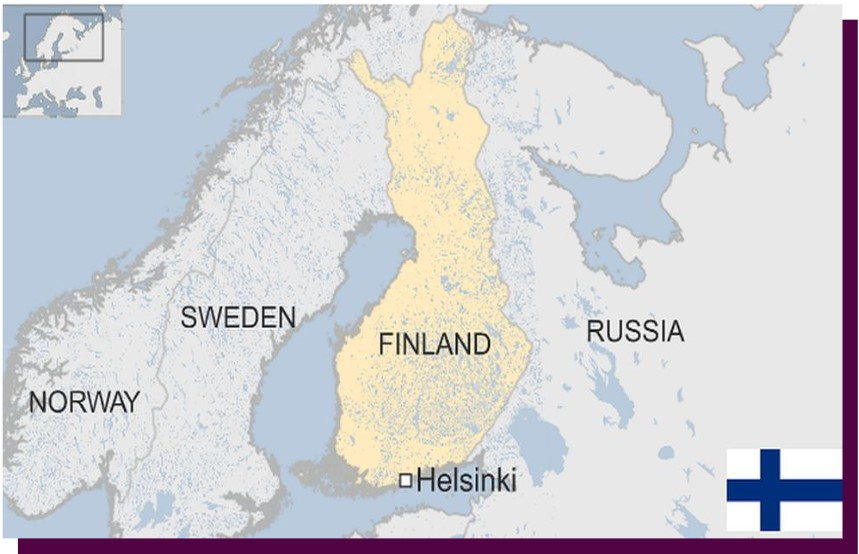
\includegraphics[scale=.35]{img/fig16.jpg}
\end{minipage}

\begin{minipage}{\textwidth}
    \footnotesize{
    \begin{itemize}
        \item Resilience building program relies on formal education and is reported to be among the most successful in the world with the highest Media Literacy Index score in Europe
        \item The score reflects a discerning population that scrutinizes the source of information.
        \item This does not mean Finns believe everything they read in the papers and never look at social media for information. But when they do, most have the ability to critically evaluate information.
    \end{itemize}
    }
\end{minipage}

\note[]{
-Erica Benke and Marianna Spring, “US Midterm Elections: Does Finland Have the Answer to Fake News?,” \emph{BBC News}, October 12, 2022, sec. Europe, \url{https://www.bbc.com/news/world-europe-63222819.}
-“Countries and Territories,” Freedom House, accessed January 2, 2023, https://freedomhouse.org/countries/freedom-world/scores.

}
\end{frame}


%%%%%%%%%%%%%%%%%%%%%%%%%%%%%%%%%%%%%%%%%%%%%%%%
%%%%%%%%%%%%%%%%  SLIDE 14  %%%%%%%%%%%%%%%%%%%%%
%%%%%%%%%%%%%%%%%%%%%%%%%%%%%%%%%%%%%%%%%%%%%%%%
\begin{frame}{Lithuania}
\begin{minipage}{\textwidth}
    \centering 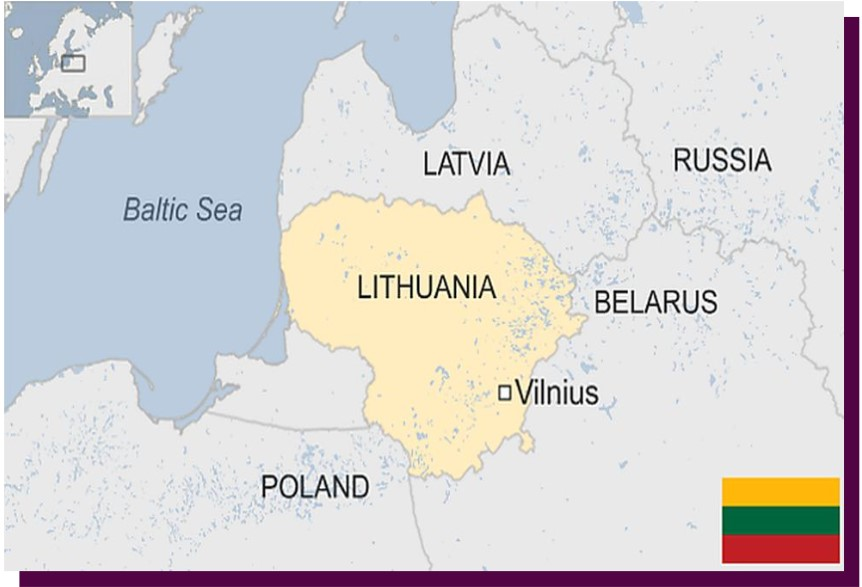
\includegraphics[scale=.35]{img/fig17.jpg}
\end{minipage}

\begin{minipage}{\textwidth}
    \footnotesize{
    \begin{itemize}
        \item 5000 volunteers called Elves cull through and report on the accuracy of thousands of stories per year.  The stories are passed to the Elves in several ways.
        \item One of the primary conduits is from debunk.eu.  Debunk.eu is an advanced platform using algorithms designed to spot disinformation almost as soon as it is generated. 
        \item Should the Elves determine a story is likely disinformation, they pass it to local journalists.  Journalists review the reports and, at times, will publish stories.
        \item In the background are academics, the Ministry of Foreign Affairs, and the military.  These three entities provide support, intelligence, and expertise to the Elves, debunk.eu, and the journalists
    \end{itemize}
    }
\end{minipage}

\note[]{
-Content Commons. “A Counter-Disinformation System That Works,” February 20, 2020. \url{https://commons.america.gov/article?id=44\&site=content.america.gov.}
}
\end{frame}


%%%%%%%%%%%%%%%%%%%%%%%%%%%%%%%%%%%%%%%%%%%%%%%%
%%%%%%%%%%%%%%%%  SLIDE 15  %%%%%%%%%%%%%%%%%%%%%
%%%%%%%%%%%%%%%%%%%%%%%%%%%%%%%%%%%%%%%%%%%%%%%%
\begin{frame}{Estonia}
\begin{minipage}{\textwidth}
    \centering 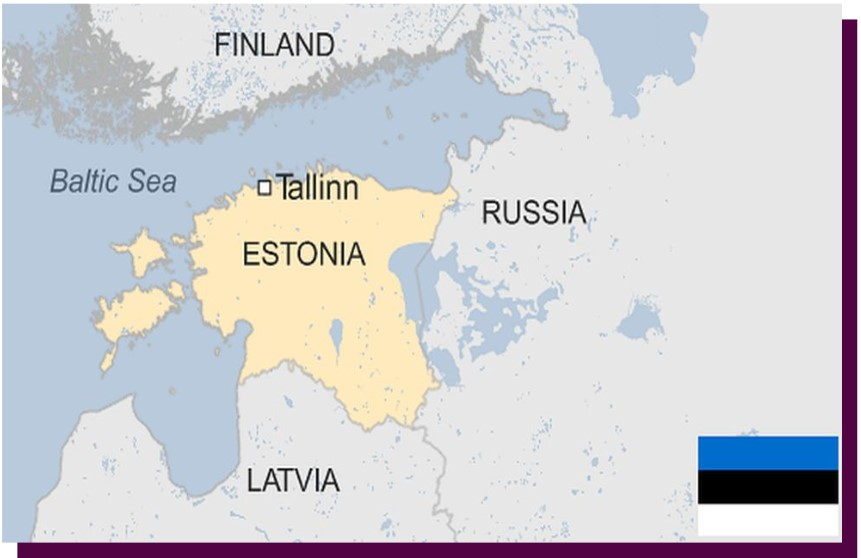
\includegraphics[scale=.35]{img/fig18.jpg}
\end{minipage}

\begin{minipage}{\textwidth}
    \footnotesize{
    \begin{itemize}
        \item Estonia has a sizeable ethnic Russian population which makes up a quarter of the population
        \item Estonia’s Defense League (EDL) is under the Ministry of Defense but staffed primarily by civilian volunteers. 
        \item EDL’s mission is to locate, expose, and counter disinformation
        \item Like the Lithuanians, the EDL utilizes elves and a technical platform, Propastop.org, to work its mission
    \end{itemize}
    }
\end{minipage}

\note[]{
-Robbins, Joseph. “Countering Russian Disinformation,” September 23, 2020, \url{https://www.csis.org/blogs/post-soviet-post/countering-russian-disinformation}
}
\end{frame}

%%%%%%%%%%%%%%%%%%%%%%%%%%%%%%%%%%%%%%%%%%%%%%%%
%%%%%%%%%%%%%%%%  SLIDE 16  %%%%%%%%%%%%%%%%%%%%%
%%%%%%%%%%%%%%%%%%%%%%%%%%%%%%%%%%%%%%%%%%%%%%%%
\begin{frame}{Class Questions}

\begin{minipage}{0.5\textwidth}
    \footnotesize{
        Strategies from social media and governmental organizations for identifying, tracking and countering mis and disinformation.
        \begin{itemize}
            \item Consider the United States? 
            \item All of the above-listed countries score better than the U.S. of democracy and freedom scores 
            \item The U.S. funds overseas efforts to spot and counter mis/disinformaiton at a much higher amount than it does domestically
            \item Could one of these European programs be utilized in the U.S., why, or why not?
        \end{itemize}
    }
\end{minipage}
\hspace{0.05\textwidth}
\begin{minipage}{0.42\textwidth}
\footnotesize{ \raggedright{
    Additional Reading: \newline 
    
    Content Commons. “A Counter-Disinformation System That Works,” February 20, 2020. \href{https://commons.america.gov/article?id=44\&site=content.america.gov.}{https://commons.america.gov...} \newline 
    
    Robbins, Joseph. “Countering Russian Disinformation,” September 23, 2020, }\href{https://www.csis.org/blogs/post-soviet-post/countering-russian-disinformation}{https://www.csis.org/blogs/post-soviet-post/countering-russian-disinformation.}
}
\end{minipage}
\note[]{

}
\end{frame}

%%%%%%%%%%%%%%%%%%%%%%%%%%%%%%%%%%%%%%%%%%%%%%%%
%%%%%%%%%%%%%%%%  SLIDE 17  %%%%%%%%%%%%%%%%%%%%%
%%%%%%%%%%%%%%%%%%%%%%%%%%%%%%%%%%%%%%%%%%%%%%%%
\begin{frame}{}

\begin{minipage}{0.4\textwidth}
    \raggedright\Large{\textbf{Demand for Misinformation/
                                Disinformation/
                                Propaganda
    }}
\end{minipage}
\hspace{0.05\textwidth}
\begin{minipage}{0.5\textwidth}

    \begin{itemize}
    \small{
        \item Social Identity
        \item Avoidance of cognitive dissonance
        \item Heuristics

    }
    \end{itemize}
\end{minipage}
\end{frame}


%%%%%%%%%%%%%%%%%%%%%%%%%%%%%%%%%%%%%%%%%%%%%%%%
%%%%%%%%%%%%%%%%  SLIDE 18  %%%%%%%%%%%%%%%%%%%%%
%%%%%%%%%%%%%%%%%%%%%%%%%%%%%%%%%%%%%%%%%%%%%%%%
\begin{frame}{Why do information / rumors / conspiracy theories resonate?}

\begin{itemize}
    \item Partisanship congruence is one of the leading predictors of belief in false information
    \item Partisan identities alter information processing linked to reasoning, memory, implicit evaluation, and even perception.

\end{itemize}

\note[]{
    \begin{enumerate}
        \item Partisanship heavily outweighs other factors such as media literacy, age, cognitive reflection, or gender that correlate with belief in misinformation
        \begin{enumerate}[a]
            \item Those that self-identify as male are more likely to believe misinformation
            \item Those younger are more likely to believe misinformation
            \item Those with lower levels of media literacy are more likely to believe misinformation
            \item Those with lower levels of cognitive reflection are more likely to believe misinformation
        \end{enumerate}

    \end{enumerate}
    Education or income levels do not appear to correlate with belief in misinformation.
}
\end{frame}


%%%%%%%%%%%%%%%%%%%%%%%%%%%%%%%%%%%%%%%%%%%%%%%%
%%%%%%%%%%%%%%%%  SLIDE 19  %%%%%%%%%%%%%%%%%%%%%
%%%%%%%%%%%%%%%%%%%%%%%%%%%%%%%%%%%%%%%%%%%%%%%%
\begin{frame}{Social Identity Theory}

\begin{itemize}
    \item Evolutionary theory has argued that the brain evolved to detect coalitional alliances.
    \item People behave and experience emotions in ways that are congruent with the activated social identity, in some cases, political affiliation.
    \item Social identities have been shown to shape the way people interpret information.
\end{itemize}
\end{frame}


%%%%%%%%%%%%%%%%%%%%%%%%%%%%%%%%%%%%%%%%%%%%%%%%
%%%%%%%%%%%%%%%%  SLIDE 20  %%%%%%%%%%%%%%%%%%%%%
%%%%%%%%%%%%%%%%%%%%%%%%%%%%%%%%%%%%%%%%%%%%%%%%
\begin{frame}{Social Identity Theory}

\begin{itemize}
    \item Partisan identities fulfill basic social needs such as belonging, distinctiveness, and epistemic closure.
    \item This can generate a powerful incentive to distort beliefs in a manner that defies truth – especially when the net value of these goals outweighs accuracy goals.

\end{itemize}
\end{frame}


%%%%%%%%%%%%%%%%%%%%%%%%%%%%%%%%%%%%%%%%%%%%%%%%
%%%%%%%%%%%%%%%%  SLIDE 21  %%%%%%%%%%%%%%%%%%%%%
%%%%%%%%%%%%%%%%%%%%%%%%%%%%%%%%%%%%%%%%%%%%%%%%
\begin{frame}{Cognitive Dissonance is Avoided}

\begin{itemize}
    \item When different beliefs are in conflict with one another, people experience an uncomfortable cognitive state – known as cognitive dissonance.
    \item Because cognitive dissonance is aversive, people are motivated to reduce that experience.
\end{itemize}
\end{frame}


%%%%%%%%%%%%%%%%%%%%%%%%%%%%%%%%%%%%%%%%%%%%%%%%
%%%%%%%%%%%%%%%%  SLIDE 22  %%%%%%%%%%%%%%%%%%%%%
%%%%%%%%%%%%%%%%%%%%%%%%%%%%%%%%%%%%%%%%%%%%%%%%
\begin{frame}{Cognitive Dissonance is Avoided}

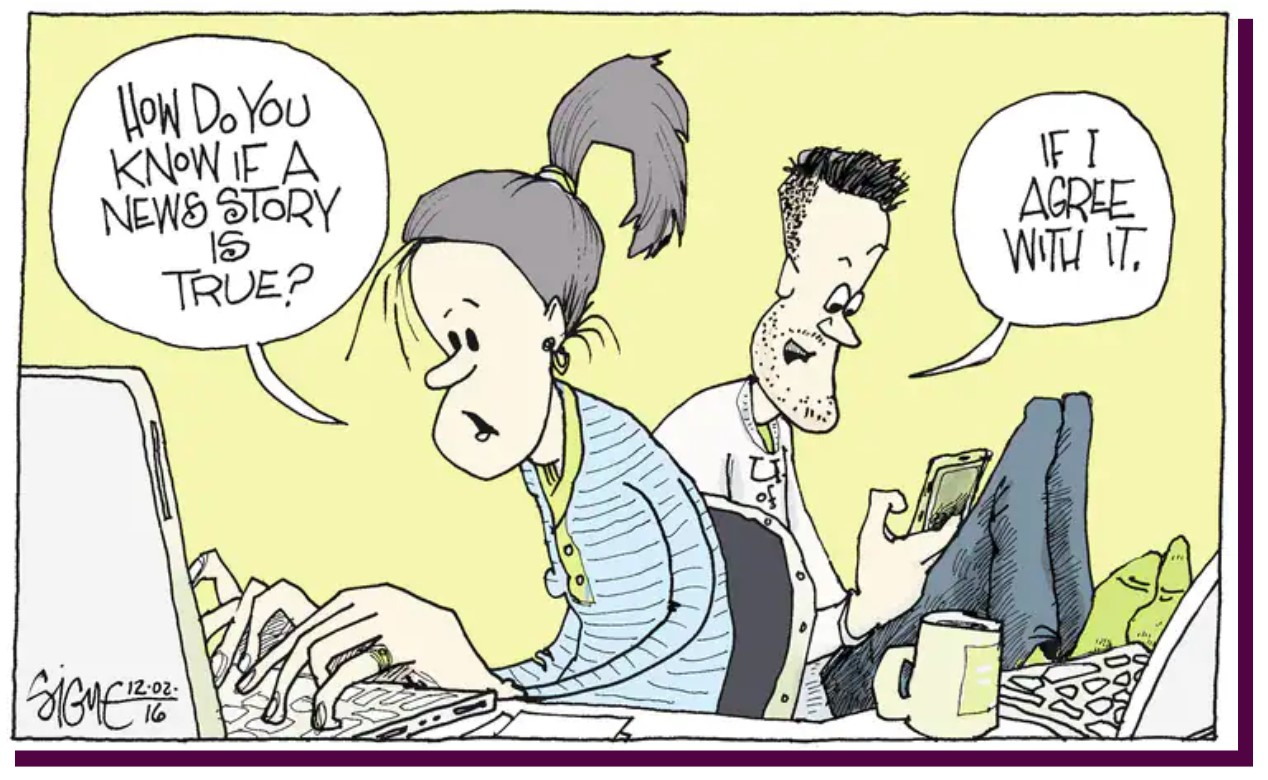
\includegraphics[width=\textwidth]{img/fig6.jpg}

\end{frame}


%%%%%%%%%%%%%%%%%%%%%%%%%%%%%%%%%%%%%%%%%%%%%%%%
%%%%%%%%%%%%%%%%  SLIDE 23  %%%%%%%%%%%%%%%%%%%%%
%%%%%%%%%%%%%%%%%%%%%%%%%%%%%%%%%%%%%%%%%%%%%%%%
\begin{frame}{Social Identity Over Accuracy}

The brain may allow highly identified individuals to value the outcomes of in-group members and engage in cognition and action consistent with their identity goals over accuracy goals. 

\end{frame}


%%%%%%%%%%%%%%%%%%%%%%%%%%%%%%%%%%%%%%%%%%%%%%%%
%%%%%%%%%%%%%%%  SLIDE 24  %%%%%%%%%%%%%%%%%%%%%
%%%%%%%%%%%%%%%%%%%%%%%%%%%%%%%%%%%%%%%%%%%%%%%%
\begin{frame}{Two Explanations for Partisan Belief in False Information}

\begin{itemize}
    \item \textbf{Heuristics}: People use information about party endorsement of particular attitudes, beliefs, or policies as cues that guide their own position either directly through low-effort strategies.
    \item \textbf{Social Identity Protection}: Making judgments that are aligned with one’s political identity is more important than achieving accuracy
\end{itemize}
    
\end{frame}

%%%%%%%%%%%%%%%%%%%%%%%%%%%%%%%%%%%%%%%%%%%%%%%%
%%%%%%%%%%%%%%%  SLIDE 25  %%%%%%%%%%%%%%%%%%%%%
%%%%%%%%%%%%%%%%%%%%%%%%%%%%%%%%%%%%%%%%%%%%%%%%
\begin{frame}{How can we reduce these partisan biases in processing Information?}

\begin{itemize}
    \item \textbf{Fulfill social needs through nonpartisan means}
    \item \textbf{Motivate people to search for the truth}: This increases the strength of accuracy goals and will reduce partisan bias.
    \item \textbf{Providing broad context}: Enriching corrective information so as to provide a broader account of the news is more likely to change false beliefs about an event.
    \item \textbf{Emphasizing Accuracy as a goal}: Prompting an accuracy goal to reach a correct conclusion can elicit greater cognitive effort towards that goal.
    \item \textbf{Appealing to a superordinate identity, such as Americans or human beings}

\end{itemize}

\note[]{

}
    
\end{frame}

%%%%%%%%%%%%%%%%%%%%%%%%%%%%%%%%%%%%%%%%%%%%%%%%
%%%%%%%%%%%%%%%  SLIDE 26  %%%%%%%%%%%%%%%%%%%%%
%%%%%%%%%%%%%%%%%%%%%%%%%%%%%%%%%%%%%%%%%%%%%%%%
\begin{frame}{}
\begin{minipage}{0.4\textwidth}
    \raggedright\Large{\textbf{Interventions designed to mitigate misinformation
    }}
\end{minipage}
\hspace{0.05\textwidth}
\begin{minipage}{0.5\textwidth}

    \begin{itemize}
        \item Individual-Level Interventions
        \item Systemic-Level Interventions
    \end{itemize}
\end{minipage}
\end{frame}



%%%%%%%%%%%%%%%%%%%%%%%%%%%%%%%%%%%%%%%%%%%%%%%%
%%%%%%%%%%%%%%%  SLIDE 27  %%%%%%%%%%%%%%%%%%%%%
%%%%%%%%%%%%%%%%%%%%%%%%%%%%%%%%%%%%%%%%%%%%%%%%
\begin{frame}{Individual-Level Interventions}

\begin{itemize}
    \item Boosting
    \item Nudging
    \item Debunking
    \item Automated content labeling
\end{itemize}
    
\end{frame}


%%%%%%%%%%%%%%%%%%%%%%%%%%%%%%%%%%%%%%%%%%%%%%%%
%%%%%%%%%%%%%%%  SLIDE 28  %%%%%%%%%%%%%%%%%%%%%
%%%%%%%%%%%%%%%%%%%%%%%%%%%%%%%%%%%%%%%%%%%%%%%%
\begin{frame}{Individual-Level Interventions
(Boosting)}

\begin{itemize}
    \item Improve individual's ability to identify misinformation. \newline 
\end{itemize}

\textbf{Examples}: Pre-bunking/inoculation, increasing critical thinking, and increasing media literacy.
    
\end{frame}



%%%%%%%%%%%%%%%%%%%%%%%%%%%%%%%%%%%%%%%%%%%%%%%%
%%%%%%%%%%%%%%%  SLIDE 29  %%%%%%%%%%%%%%%%%%%%%
%%%%%%%%%%%%%%%%%%%%%%%%%%%%%%%%%%%%%%%%%%%%%%%%
\begin{frame}{Pre-Bunking - Inoculation}


\includegraphics[width=\textwidth]{img/fig7.jpg}

\begin{center}
\underline{\textbf{\href{https://www.getbadnews.com/books/english/}{Bad News Game}}}
\end{center}

\note[]{
Pre-bunking intervention
} 
\end{frame}



%%%%%%%%%%%%%%%%%%%%%%%%%%%%%%%%%%%%%%%%%%%%%%%%
%%%%%%%%%%%%%%%  SLIDE 30 %%%%%%%%%%%%%%%%%%%%%
%%%%%%%%%%%%%%%%%%%%%%%%%%%%%%%%%%%%%%%%%%%%%%%%
\begin{frame}{Individual-Level Interventions
(Nudging Interventions)}
Shift people’s attention towards accuracy, thus reducing the likelihood they share misinformation with others.

\textbf{Examples}: Accuracy primes and social-norms nudges.
    
\end{frame}


%%%%%%%%%%%%%%%%%%%%%%%%%%%%%%%%%%%%%%%%%%%%%%%%
%%%%%%%%%%%%%%%  SLIDE 31  %%%%%%%%%%%%%%%%%%%%%
%%%%%%%%%%%%%%%%%%%%%%%%%%%%%%%%%%%%%%%%%%%%%%%%
\begin{frame}{Individual-Level Interventions
(Debunking)}
\begin{minipage}{0.37\textwidth}
    \raggedright{
    \footnotesize{
        Correcting misperceptions after they have spread \newline 

        \textbf{Examples}: Fact-checking and corrections.
    }}
\end{minipage}
\hspace{0.02\textwidth}
\begin{minipage}{0.58\textwidth}
    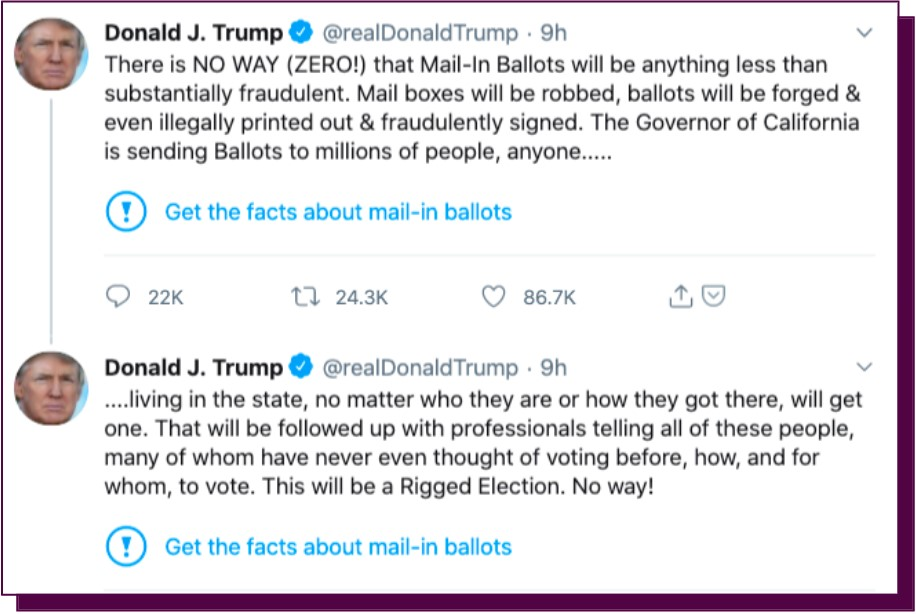
\includegraphics[width=\textwidth]{img/fig8.jpg}
\end{minipage}
    
\end{frame}


%%%%%%%%%%%%%%%%%%%%%%%%%%%%%%%%%%%%%%%%%%%%%%%%
%%%%%%%%%%%%%%%  SLIDE 32  %%%%%%%%%%%%%%%%%%%%%
%%%%%%%%%%%%%%%%%%%%%%%%%%%%%%%%%%%%%%%%%%%%%%%%
\begin{frame}{Individual-Level Interventions
(Automated Content Labeling)}
\begin{minipage}{0.37\textwidth}
    \raggedright{
    \footnotesize{
        The use of automation to quickly label content at scale. \newline 

        \textbf{Examples}: Automated or manual fact-checking labels, content warnings, or credibility labels.
    }}
\end{minipage}
\hspace{0.02\textwidth}
\begin{minipage}{0.58\textwidth}
    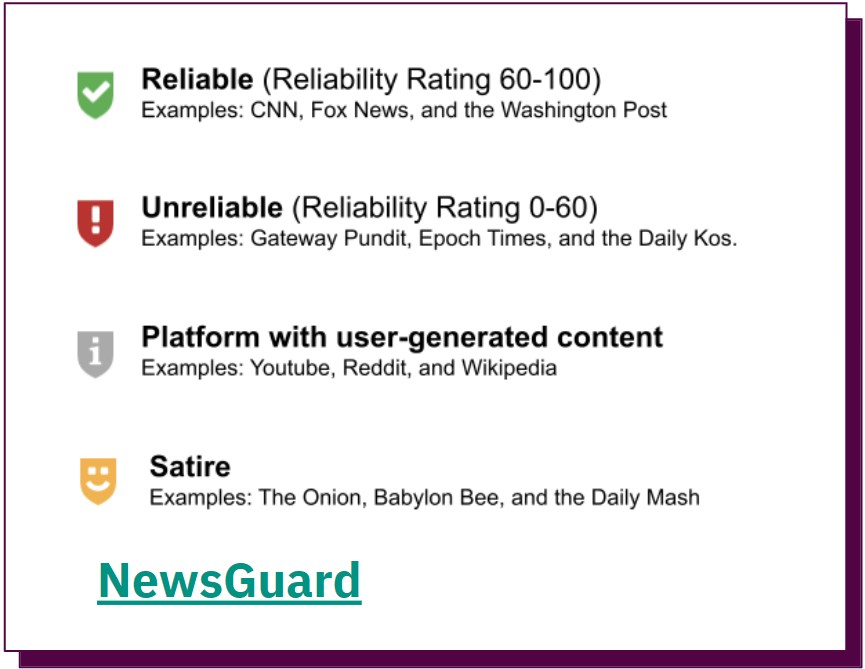
\includegraphics[width=\textwidth]{img/fig9.jpg}
\end{minipage}


\note[]{
Figure comes from: \href{https://www.science.org/doi/10.1126/sciadv.abl3844}{https://www.science.org/doi/10.1126/sciadv.abl3844}
}
    
\end{frame}


%%%%%%%%%%%%%%%%%%%%%%%%%%%%%%%%%%%%%%%%%%%%%%%%
%%%%%%%%%%%%%%%  SLIDE 33  %%%%%%%%%%%%%%%%%%%%%
%%%%%%%%%%%%%%%%%%%%%%%%%%%%%%%%%%%%%%%%%%%%%%%%
\begin{frame}{}
\begin{center}
    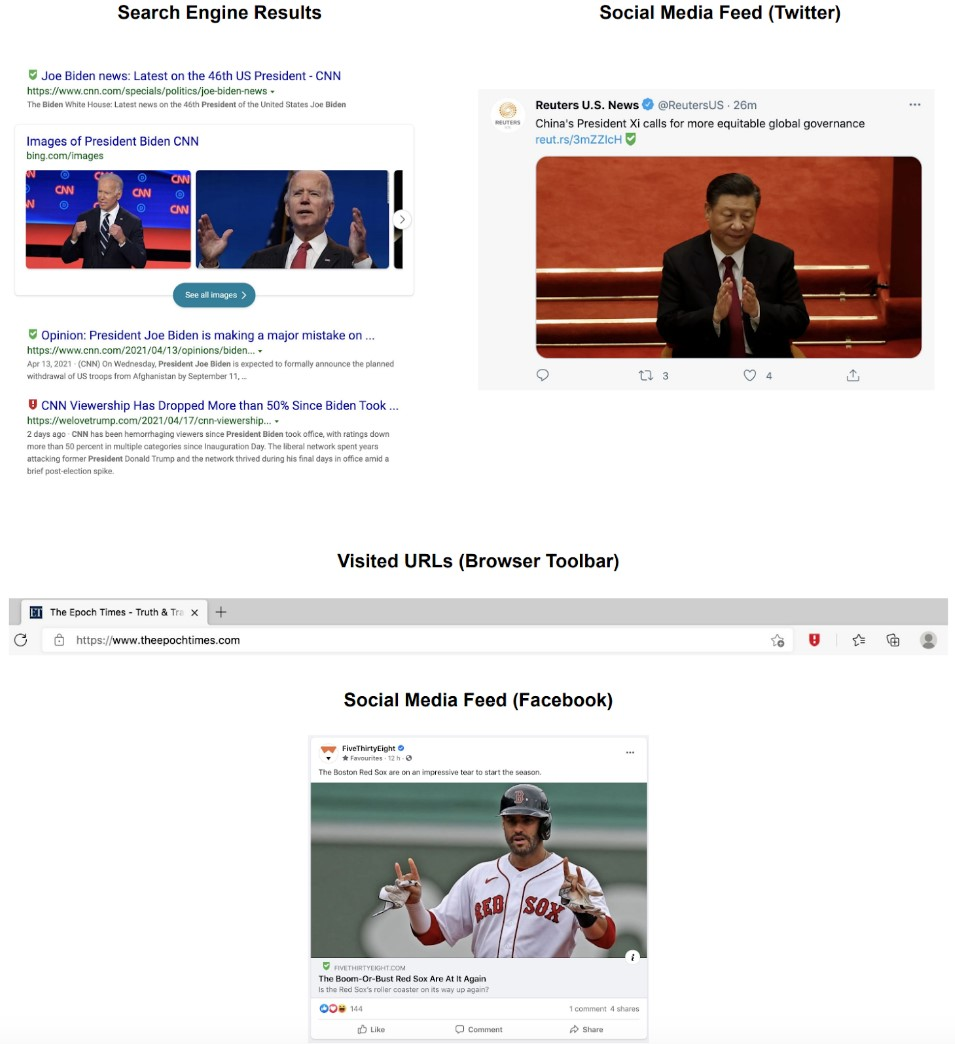
\includegraphics[scale=.4]{img/fig10.jpg}
    \footnotesize{\textbf{\underline{\href{https://www.newsguardtech.com/}{NewsGuard}}}}
\end{center}

\note[]{
Figure comes from: \href{https://www.science.org/doi/10.1126/sciadv.abl3844}{https://www.science.org/doi/10.1126/sciadv.abl3844}
}
    
\end{frame}



%%%%%%%%%%%%%%%%%%%%%%%%%%%%%%%%%%%%%%%%%%%%%%%%
%%%%%%%%%%%%%%%  SLIDE 34  %%%%%%%%%%%%%%%%%%%%%
%%%%%%%%%%%%%%%%%%%%%%%%%%%%%%%%%%%%%%%%%%%%%%%%
\begin{frame}{Path Forward on Individual-level interventions}

\begin{itemize}
    \item Test interventions in the non-western and non-english speaking world.
    \item Intervention efficacy in the lab does not always translate to the real-world.
    \item Measure how interventions work together rather than solely in isolation.
    \item Open access data from social media companies is necessary.
    \item Requiring social media companies to give insight into their platforms’ recommender algorithms is necessary.
    \item More transparency about tech companies’ efforts to measure the efficacy of their own interventions.
\end{itemize}
    
\end{frame}


%%%%%%%%%%%%%%%%%%%%%%%%%%%%%%%%%%%%%%%%%%%%%%%%
%%%%%%%%%%%%%%%  SLIDE 35  %%%%%%%%%%%%%%%%%%%%%
%%%%%%%%%%%%%%%%%%%%%%%%%%%%%%%%%%%%%%%%%%%%%%%%
\begin{frame}{Systemic-Level Interventions}

\begin{itemize}
    \item Algorithms
    \item Business Models
    \item Legislation
    \item Geopolitics
\end{itemize}
    
\end{frame}


%%%%%%%%%%%%%%%%%%%%%%%%%%%%%%%%%%%%%%%%%%%%%%%%
%%%%%%%%%%%%%%%  SLIDE 36  %%%%%%%%%%%%%%%%%%%%%
%%%%%%%%%%%%%%%%%%%%%%%%%%%%%%%%%%%%%%%%%%%%%%%%
\begin{frame}{Systemic-Level Interventions
(Algorithms)
}
\begin{center}
    \begin{minipage}{.6\textwidth}
        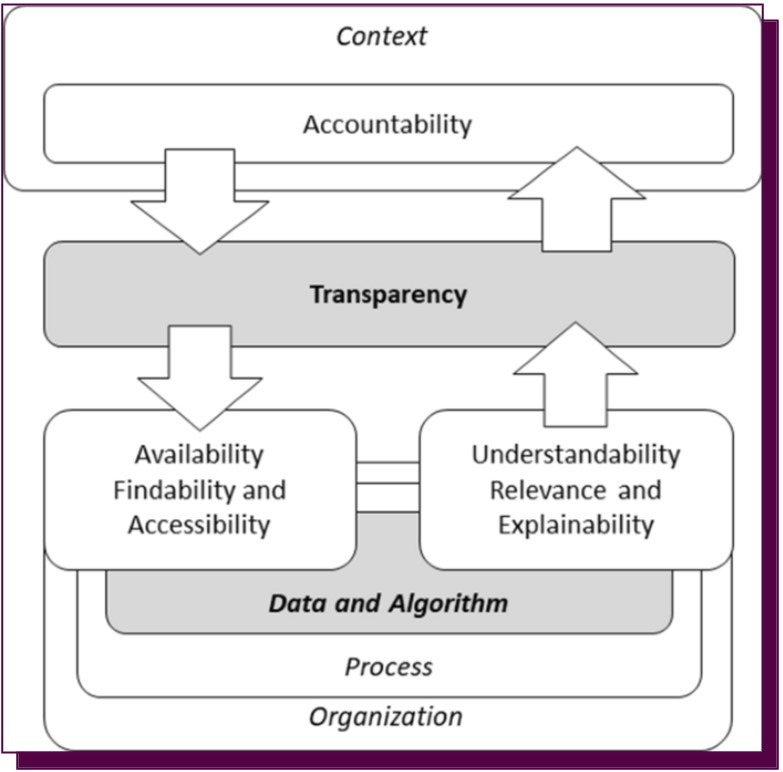
\includegraphics[width=\textwidth]{img/fig11.jpg} \newline 
    \end{minipage}
    \begin{minipage}{.6\textwidth}
        Algorithmic transparency leads to accountability
    \end{minipage}
\end{center}

\note[]{
Figure comes from: Roozenbeek, J., Suiter, J., \& Culloty, E. (2022). Countering misinformation: Evidence, knowledge gaps, and implications of current interventions.
}
    
\end{frame}


%%%%%%%%%%%%%%%%%%%%%%%%%%%%%%%%%%%%%%%%%%%%%%%%
%%%%%%%%%%%%%%%  SLIDE 37  %%%%%%%%%%%%%%%%%%%%%
%%%%%%%%%%%%%%%%%%%%%%%%%%%%%%%%%%%%%%%%%%%%%%%%
\begin{frame}{Systemic-Level Interventions
(Business Models)}

Addressing ad-tech and supporting reliable media.

\end{frame}


%%%%%%%%%%%%%%%%%%%%%%%%%%%%%%%%%%%%%%%%%%%%%%%%
%%%%%%%%%%%%%%%  SLIDE 38  %%%%%%%%%%%%%%%%%%%%%
%%%%%%%%%%%%%%%%%%%%%%%%%%%%%%%%%%%%%%%%%%%%%%%%
\begin{frame}{}

\begin{center}
    \begin{minipage}{.8\textwidth}
        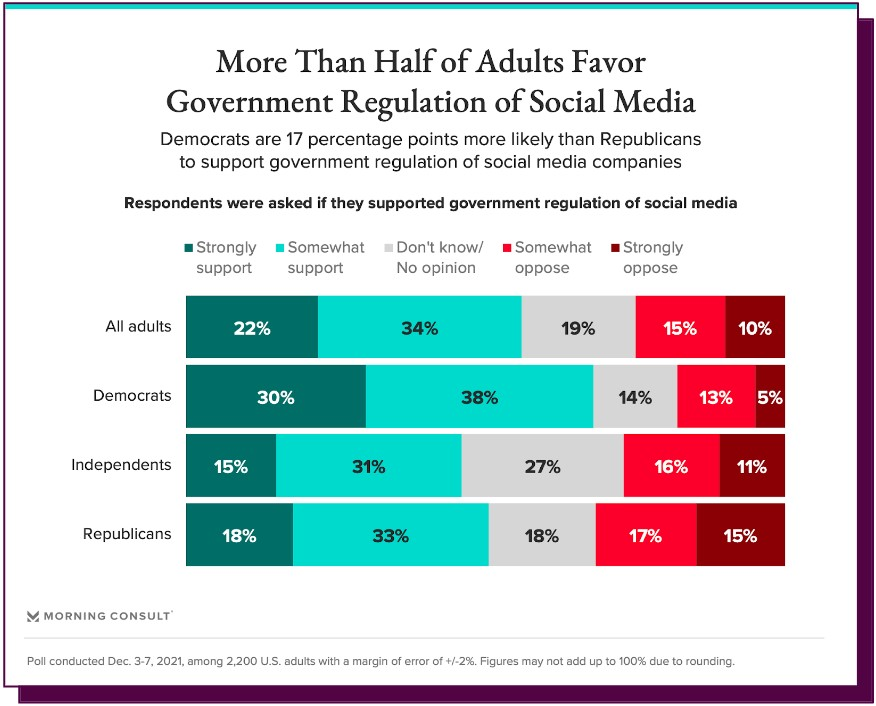
\includegraphics[width=\textwidth]{img/fig12.jpg} \newline 
    \end{minipage}
    \begin{minipage}{.4\textwidth}
        \small{Regulating tech platforms.}
    \end{minipage}
\end{center}

\note[]{
Figure comes from: \href{https://morningconsult.com/2021/12/15/social-media-regulation-poll-2022/}{https://morningconsult.com/2021/12/15/social-media-regulation-poll-2022/}
}
    
\end{frame}


%%%%%%%%%%%%%%%%%%%%%%%%%%%%%%%%%%%%%%%%%%%%%%%%
%%%%%%%%%%%%%%%  SLIDE 39  %%%%%%%%%%%%%%%%%%%%%
%%%%%%%%%%%%%%%%%%%%%%%%%%%%%%%%%%%%%%%%%%%%%%%%
\begin{frame}{Systemic-Level Interventions
(Geopolitics)}

\begin{center}
    \begin{minipage}{.8\textwidth}
        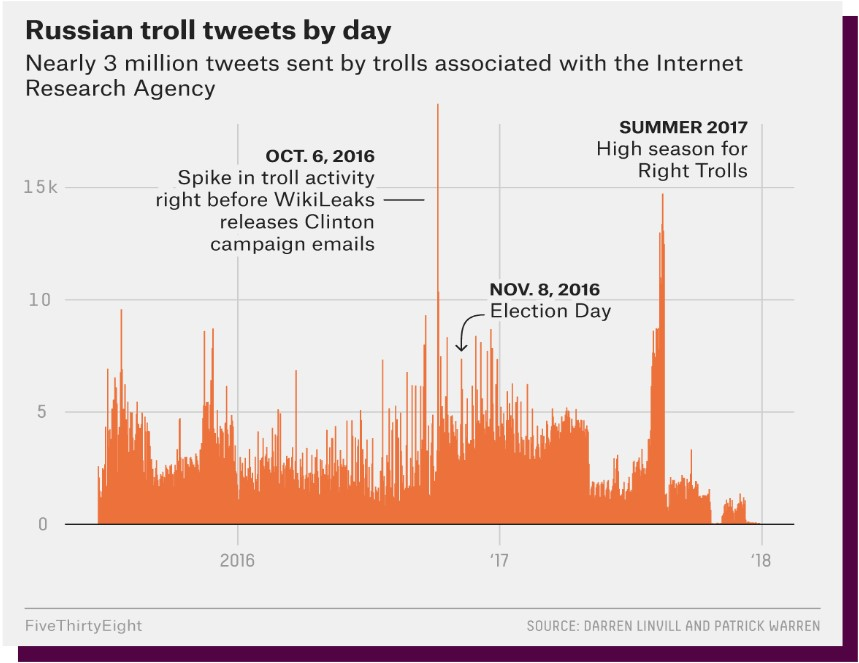
\includegraphics[width=\textwidth]{img/fig13.jpg} \newline 
    \end{minipage}
    \begin{minipage}{.4\textwidth}
        \footnotesize{Combating nefarious actors and reducing polarization.}
    \end{minipage}
\end{center}


\note[]{
The figure is pulled from this FiveThirtyEight piece: \href{https://fivethirtyeight.com/features/why-were-sharing-3-million-russian-troll-tweets/}{https://fivethirtyeight.com/features/why-were-sharing-3-million-russian-troll-tweets/}
}
    
\end{frame}

%%%%%%%%%%%%%%%%%%%%%%%%%%%%%%%%%%%%%%%%%%%%%%%%
%%%%%%%%%%%%%%%  SLIDE 40  %%%%%%%%%%%%%%%%%%%%%
%%%%%%%%%%%%%%%%%%%%%%%%%%%%%%%%%%%%%%%%%%%%%%%%
\begin{frame}{}

\begin{minipage}{0.4\textwidth}
    \raggedright\Large{\textbf{Supply-side of Misinformation/
                                Disinformation/
                                Propaganda
    }}
\end{minipage}
\hspace{0.05\textwidth}
\begin{minipage}{0.5\textwidth}

    \begin{itemize}
    \small{
        \item How do disinformation campaigns operate on social media? \newline 

        \item How do Authoritarian State Actors Spread Propaganda?


    }
    \end{itemize}
\end{minipage}

\note[]{

}
    
\end{frame}


%%%%%%%%%%%%%%%%%%%%%%%%%%%%%%%%%%%%%%%%%%%%%%%%
%%%%%%%%%%%%%%%  SLIDE 41  %%%%%%%%%%%%%%%%%%%%%
%%%%%%%%%%%%%%%%%%%%%%%%%%%%%%%%%%%%%%%%%%%%%%%%
\begin{frame}{How do disinformation campaigns operate on social media?}

\begin{itemize}
    \item Disinformation campaigns purposely entangle orchestrated action with organic activity, not just trolls.
    \item Disinformation often layers true information with false information making it difficult to label as blatantly false.
    \item Disinformation is sometimes designed to overwhelm our capacity to make sense of information and to encourage us to disengage.
\end{itemize}
    
\end{frame}



%%%%%%%%%%%%%%%%%%%%%%%%%%%%%%%%%%%%%%%%%%%%%%%%
%%%%%%%%%%%%%%%  SLIDE 42  %%%%%%%%%%%%%%%%%%%%%
%%%%%%%%%%%%%%%%%%%%%%%%%%%%%%%%%%%%%%%%%%%%%%%%
\begin{frame}{How do disinformation campaigns operate on social media?}

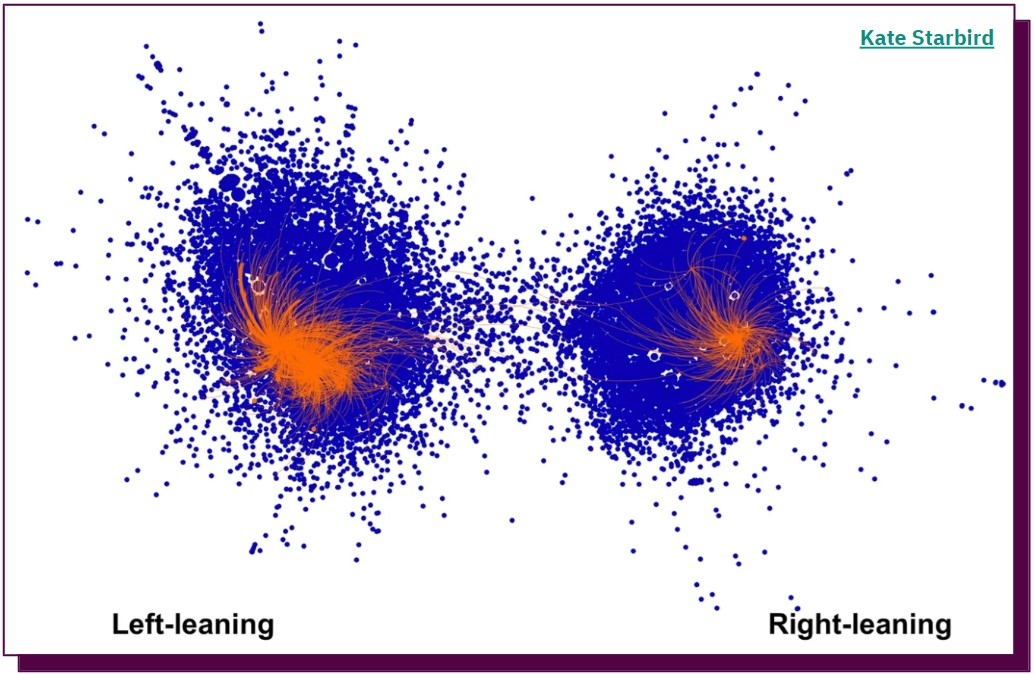
\includegraphics[width=\textwidth]{img/fig14.jpg}

\note[]{
\footnotesize{
To understand how IRA accounts participated in the \#BlackLivesMatter Twitter conversation, Kate Starbird and co-authors a network graph using retweet patterns from Twitter accounts using the hashtag. Two different clusters of accounts tended to retweet other accounts in their cluster, but not accounts in the other cluster.There was a cluster of accounts (on the left) that was pro-BlackLivesMatter and liberal/Democrat and a cluster (on the right) that was anti-BlackLivesMatter and conservative/Republican. They then identified and highlighted the accounts identified as part of the IRA’s information operations on Twitter during the Black Lives Matter protests. That graph is pictured here, with the IRA accounts in orange and other accounts in blue. As you can see, the IRA accounts impersonated activists on both sides of the conversation. \newline 

This comes from: \href{https://medium.com/s/story/the-trolls-within-how-russian-information-operations-infiltrated-online-communities-691fb969b9e4}{https://medium.com/s/story/the-trolls-within-how-russian-information-operations-infiltrated-online-communities-691fb969b9e4}
}
}
    
\end{frame}



%%%%%%%%%%%%%%%%%%%%%%%%%%%%%%%%%%%%%%%%%%%%%%%%
%%%%%%%%%%%%%%%  SLIDE 43  %%%%%%%%%%%%%%%%%%%%%
%%%%%%%%%%%%%%%%%%%%%%%%%%%%%%%%%%%%%%%%%%%%%%%%
\begin{frame}{How do Authoritarian State Actors Spread Propaganda?}

\begin{itemize}
    \item Social media accounts rarely directly confront the opposition and act on the behalf of Authoritarian state actors when criticized.
    \item Rather, the strategic objective is to distract and redirect public attention from discussions or events with collective action potential.
    \item These posts engage disproportionately in cheerleading for the regime.
\end{itemize}
    
\end{frame}



%%%%%%%%%%%%%%%%%%%%%%%%%%%%%%%%%%%%%%%%%%%%%%%%
%%%%%%%%%%%%%%%  SLIDE 44  %%%%%%%%%%%%%%%%%%%%%
%%%%%%%%%%%%%%%%%%%%%%%%%%%%%%%%%%%%%%%%%%%%%%%%
\begin{frame}{How do Authoritarian State Actors Spread Propaganda?}

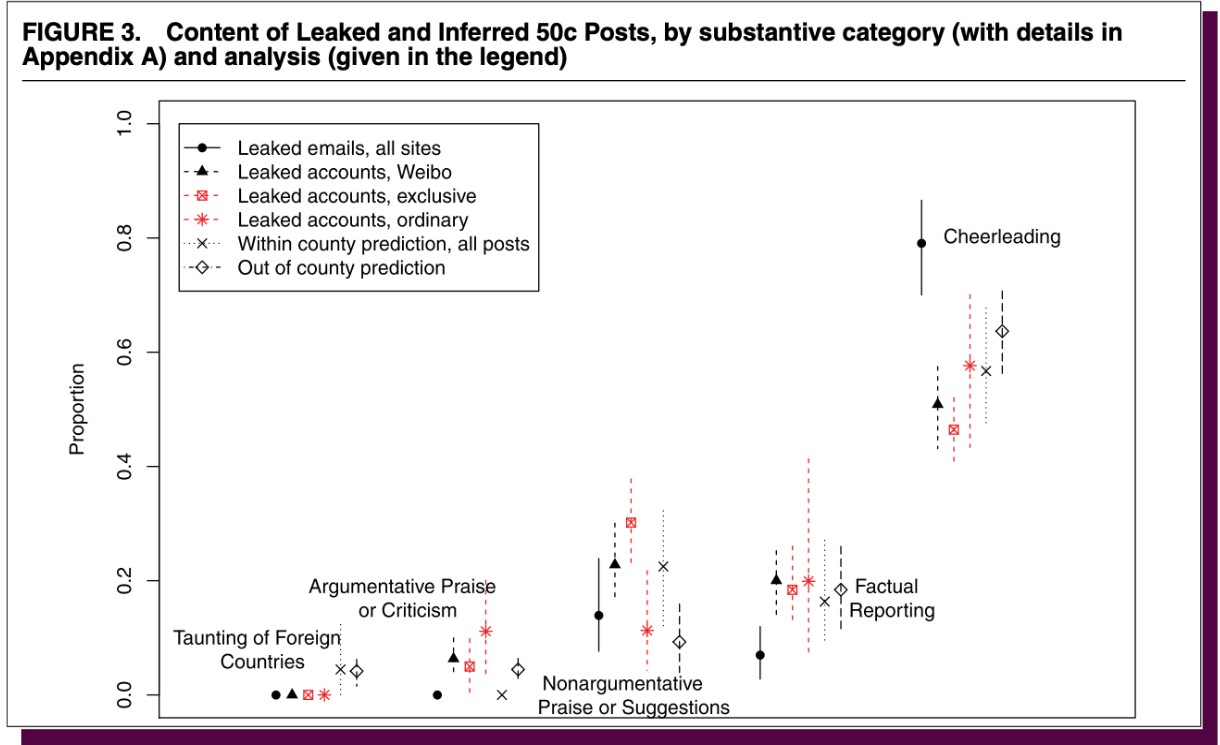
\includegraphics[width=\textwidth]{img/fig15.jpg}

\note[]{
Figure comes from: King, G., Pan, J., \& Roberts, M. E. (2017). How the Chinese government fabricates social media posts for strategic distraction, not engaged argument. American political science review, 111(3), 484-501. \href{https://www.cambridge.org/core/services/aop-cambridge-core/content/view/4662DB26E2685BAF1485F14369BD137C/S0003055417000144a.pdf/how-the-chinese-government-fabricates-social-media-posts-for-strategic-distraction-not-engaged-argument.pdf}{Accessible for free here.}
}
    
\end{frame}



%%%%%%%%%%%%%%%%%%%%%%%%%%%%%%%%%%%%%%%%%%%%%%%%
%%%%%%%%%%%%%%%  SLIDE 45  %%%%%%%%%%%%%%%%%%%%%
%%%%%%%%%%%%%%%%%%%%%%%%%%%%%%%%%%%%%%%%%%%%%%%%
\begin{frame}{Readings / References}

\begin{enumerate}
\scriptsize{
    \item Guess, A. M., \& Lyons, B. A. (2020). Misinformation, disinformation, and online propaganda. \emph{Social media and democracy: The state of the field, prospects for reform, 10}. \href{https://www.cambridge.org/core/books/social-media-and-democracy/E79E2BBF03C18C3A56A5CC393698F117}{Accessible for free here.}
    \item Kallas, Kristina. “Claiming the Diaspora: Russia’s Compatriot Policy and Its Reception by Estonian-Russian Population.” \emph{Journal on Ethnopolitics and Minority Issues in Europe 15}, no. 3 (2016): 1–25. \href{https://www.ecmi.de/fileadmin/downloads/publications/JEMIE/2016/Kallas.pdf}{https://www.ecmi.de/fileadmin/downloads/publications/JEMIE/2016/Kallas.pdf.}
    \item Rossbach, Niklas H. “Psychological Defense:  Vital for Sweden’s Capability.” \emph{Strategic Outlook 7} (November 2017). 
    \item Van Bavel, J. J., \& Pereira, A. (2018). The partisan brain: An identity-based model of political belief. \emph{Trends in cognitive sciences, 22(3)}, 213-224.
    \item Roozenbeek, J., Suiter, J., \& Culloty, E. (2022). Countering misinformation: Evidence, knowledge gaps, and implications of current interventions. \href{https://psyarxiv.com/b52um}{Accessible for free here.}
    \item Starbird, K. (2019). Disinformation's spread: bots, trolls and all of us. \emph{Nature, 571}(7766), 449-450.\href{https://www.nature.com/articles/d41586-019-02235-x}{Accessible for free here.} 
    \item King, G., Pan, J., \& Roberts, M. E. (2017). How the Chinese government fabricates social media posts for strategic distraction, not engaged argument. \emph{American political science review, 111}(3), 484-501. \href{https://www.cambridge.org/core/services/aop-cambridge-core/content/view/4662DB26E2685BAF1485F14369BD137C/S0003055417000144a.pdf/how-the-chinese-government-fabricates-social-media-posts-for-strategic-distraction-not-engaged-argument.pdf}{Accessible for free here.}
    }
\end{enumerate}
    
\end{frame}

%\backpage

\end{document}